\chapter[Cost-based variable selection]{Cost-based variable selection to improve clinical utility of prediction models}
\label{sec:chp_varselection}

\begin{flushleft}
{\huge\sffamily In preparation}
\end{flushleft}

as: 
\begin{quote}
Barreñada L, Vickers A, Steyerberg E, Timmerman D, Wynants L, Van Calster B. Cost-based variable selection to improve clinical utility of prediction models. Diag. Prog. Res. (submitted).
\end{quote}
% \vspace{-0.5em}
% \noindent\scriptsize\textit{Submitted: X/X/X \quad Published: -- \quad APC: XXX€}
% \normalsize\vspace{-0.5em}

\section*{Summary}\label{abstract}
Clinical prediction models guide diagnostic and prognostic decision-making. However, traditional variable selection methods rely primarily on statistical properties, often ignoring clinical utility and measurement costs. This study introduces a novel variable selection algorithm that selects predictors by maximizing harm-adjusted Net Benefit (NB). By incorporating the "test tradeoff", the specific harm or clinical cost associated with measuring a predictor, into the NB calculation , the algorithm evaluates predictor subsets to identify the clinically optimal model. For high-dimensional datasets, a backward elimination extension is provided, alongside a permutation-based NB variable importance metric to guide selection when harms are difficult to quantify. Demonstrated through a real world ovarian cancer dataset, the utility-guided approach favors simpler, cost-effective models, demonstrating that statistical performance does not necessarily equate to optimal clinical cost-utility.

\newpage

\section{Introduction}

Determining a patient's condition based on their current characteristics is called diagnosis and is key to initiate any treatment and minimize future complications. Different conditions require exploring different characteristics. For example, a bone fracture can be diagnosed through medical imaging and COVID-19 through a PCR test. Clinical prediction models are statistical tools that estimate the probability that a patient has or will develop a condition in the future \cite{steyerberg2019clinical}. These models try to link the outcome (event or condition) with a series of predictors in a dataset, a task often called supervised learning \cite{jamesIntroductionStatisticalLearning2021}. These predictors should be information readily available at the time of diagnosis, not too costly to measure and measured with reasonable precision \cite{steyerberg2019clinical}. However, there might be a vast number of predictors that meet these criteria and selecting among them is needed \cite{chowdhuryVariableSelectionStrategies2020}.

Variable selection, best subset selection, feature selection, and feature engineering are terms used in prediction modelling to describe the process of selecting which predictors to use when training a model. Different approaches for variable selection have been presented. Heinze and colleagues \cite{heinzeVariableSelectionReview2018} categorized methods into five groups based on the criteria to select the variables: (1) based on significance testing, (2) based on information criteria (e.g.\ AIC, BIC), (3) based on penalized likelihood (e.g.\ LASSO, elastic-net), (4) based on change-in-estimate or performance (e.g.\ backward elimination, stepwise selection), or (5) based on background or domain knowledge. Across machine learning literature, it is often observed that variable selection methods are grouped into filter, wrapper and embedded methods \cite{Nguyen2025Vol1}. Filter methods use statistical properties to select variables and are therefore equivalent to significance testing and information criteria-based approaches. Wrapper methods, in contrast, use model performance to select the best subset, which corresponds to Heinze's change-in-estimate criterion. Finally, embedded methods perform variable selection as part of the model training; this includes penalized likelihood but also other approaches such as feature importance calculation in tree-based or genetic algorithms \cite{archerEmpiricalCharacterizationRandom2008,zhangVariableSelectionLogistic2018}. This work will focus on change-in-estimate or wrapper methods for variable selection in clinical prediction models.

To be used in clinical practice, prediction models need to show good performance in external validation in terms of discrimination (area under the ROC curve), calibration (calibration plot), and clinical utility (Net Benefit) \cite{calsterPerformanceEvaluationPredictive2024}. Variable selection is usually performed by considering only the statistical properties of the predictors (filter methods), without accounting for the clinical benefit or utility. Utility refers to the quality of decision-making when a risk model is used to decide whether a patient requires treatment \cite{vancalsterReportingInterpretingDecision2018}. Regarding model validation there is increasing awareness that classical statistical measures are insufficient \cite{steyerberg2019clinical,calsterPerformanceEvaluationPredictive2024}. Models that are not clinically useful are more likely to be forgotten quickly or even never be implemented in real practice \cite{wyattCommentaryPrognosticModels1995}. Consequently, we aim to include clinical utility in the model development process through a clinical utility guided variable selection.

Preliminary efforts to add utility to variable selection have struggled with the generation of utility values and the complexity of the methods  \cite{fouskakisBayesianVariableSelection2009}. Fouskakis and colleagues proposed using stochastic optimization to select the model with the best cost-adjusted Bayesian Information Criterion (BIC). The cost-adjusted BIC extends standard model selection by penalizing the total measurement cost of predictors rather than solely the number of variables included. However, implementing this method requires the specification of a cost-penalized prior, a task that proves difficult for clinicians who must quantify the trade-off between statistical gain and data collection burden.

Utility values, relating to misclassification costs (i.e., the benefit of treating the diseased and the harm of treating the healthy), are hard to elicit at an absolute scale. However, it is known that the ratio of harm to benefit is directly related to the risk threshold for classifying a patient as high risk \cite{vancalsterReportingInterpretingDecision2018}. Net Benefit (NB), a simple metric for clinical utility, uses this relationship. NB is calculated as benefit minus harm multiplied by the exchange rate, or harm-to-benefit ratio \cite{vickersDecisionCurveAnalysis2006}. In statistical terms, this is the number of true positives minus the number of false positives weighted by the exchange rate. This exchange rate reflects how many false positives a clinician is willing to accept per true positive. For example, if a surgeon is willing to perform 9 surgeries on benign tumors to catch 1 malignant tumor, the exchange rate is 1/9, corresponding to a 10\% risk threshold. However, NB should often be presented across a range of thresholds, given variability across clinicians and settings \cite{vickersSimpleStepbystepGuide2019}. NB is a semi-proper metric. A proper metric is one where the expected value is maximized when the model used is correct. NB is semi-proper because it can also be maximized by some incorrect models, provided the imperfect model perfectly classifies at the decision threshold \cite{calsterPerformanceEvaluationPredictive2024}. The use of NB and related metrics to evaluate a new variable was discussed by Baker and colleagues several years ago \cite{bakerEvaluatingNewMarker2012}. However, it has never been implemented as a variable selection algorithm for clinical prediction models.

The aim of this paper is therefore to develop a simple and interpretable variable selection algorithm based on clinical utility to determine the predictors to include in the model. Additionally, we will explore the effect on performance of this method with respect to traditional procedures. We will use and implement the method in the context of a logistic regression to estimate the probability of a binary outcome, but the rationale extends to more flexible machine learning or AI probabilistic algorithms.

\section{Methodology}

\subsection{Algorithm}

The problem we aim to address is defined as follows: given a set of predictors and a modelling algorithm we seek the subset of predictors that maximizes the net benefit:

\begin{equation}
\underset{\mathbf{S} \subseteq \mathbf{P}}{\operatorname{argmax}} \widehat{NB}(\mathbf{S}, \mathbf{M}, t)
\end{equation}

Here, $\widehat{NB}(\mathbf{S}, \mathbf{M}, t)$ denotes the (adjusted) net benefit of algorithm $\mathbf{M}$ with $\mathbf{S}$ predictors for the benefit-harm trade-off $t$. The $t$ parameter may be a single value, or a range of clinically relevant values specified based on clinical context. In cases where a range of values is used, we want to maximize the average NB across that range. This is the general rationale for the methodology; however, we will focus here on the specific case where a logistic regression model is used as the modelling algorithm.

The proposed variable selection algorithm does not involve modifying coefficient estimation, since the logloss minimisation (or log-likelihood maximisation) is known to provide coefficients with good properties. Therefore, the proposed algorithm works as follows:

\begin{enumerate}
\item Define all possible model combinations based on the predictors
\item Assign a test tradeoff or harm to each predictor or group of predictors to adjust the NB accordingly. If the harm is unknown, this can be 0 and unadjusted NB will be used
\item Train models and evaluate their net benefit using cross validation with folds (default is 5)
\item This step can be parallelized to reduce computation time
\item Nonlinearities can be addressed with restricted cubic splines
\item Interactions can be included; we limit this option to either all pairwise interactions or no interactions. If interactions are included:
\item Rank the models based on NB and select the model with optimal NB
\end{enumerate}

Code implementing the Net Benefit based variable selection and the associated visualizations is available in the open-source R package NBvarsel (\url{https://lasaibarrenada.github.io/NB_varsel/}, Box~1).

\begin{codebox}[Box 1: Implementing the Methodology in R]
n <- 500
df <- data.frame(
	X1 = rnorm(n),
	X2 = rbinom(n, 1, 0.7),
	X3 = rnorm(n),
	X4 = rbinom(n, 1, 0.5)
)
df$y <- rbinom(n, 1, plogis(2 + 1*df$X1 + 1.5*df$X2 + 0.2*df$X3))

## Step 1: Install the package (once)
# install.packages("NB_varsel")
library(NB_varsel)

## Step 2: (Optional) Define harms for predictors
harms <- c(X1 = 0.1, X2 = 0.05, X3 = 0.0001, X4 = 0)

## Step 3: Run the core variable-selection routine
result <- nb_varsel(
	data = df,
	outcome_var = "y",
	costs = harms,
	mode = "exhaustive",
	folds = 5,
	permutations = TRUE,
	allow_parallel = FALSE
)

## Step 4: Visualisations (built-in)
all_subset_plot(result$all_models)
VIF_plot(result$all_models, color = "darkgreen")
\end{codebox}

\subsection{Large dimensional settings}

The algorithm presented in Section~2.1 becomes computationally too demanding when the number of candidate predictors increases. For a dataset with 20 candidate predictors, there are more than one million predictor combinations; consequently, the method fits 5 million models when using 5-fold cross-validation. In most trials or observational studies, the sample size is limited; therefore, the number of candidate predictors should also be kept small. Our methodology should always be used in compliance with these sample size criteria as explained in Section~2.2. However, in those cases where the dimensionality of the data is large (e.g.\ electronic health records), we propose an extension of the methodology that we called groupwise (as opposed to exhaustive) net benefit variable selection.

In this extension, instead of calculating all the possible combinations, we use backward elimination with a number of predictors per step specified ($k$), yielding a total of $\binom{p}{k}$ model combinations per step. The fastest version ($k = 1$) therefore would fit $p$ models by removing a single predictor in the first iteration. Then the model with best performance is selected, if that model is the model where all predictors are used, that is selected as the best model, else the predictor(s) that were removed in the model with best performance are removed and the process is iteratively repeated until reaching the optimal model. Allowing values of $k$ higher than one is highly recommended if there is intuition of important interaction effects between predictors.

\subsection{Note on Sample size}

Across systematic reviews of prediction model development and validation studies, a common issue is that there is no rationale for the sample size used \cite{barrenadaADNEXRiskPrediction2024,wynantsPredictionModelsDiagnosis2020}. International guidelines for prediction modelling, such as TRIPOD+AI and PROBAST+AI, recommend always justifying sample size \cite{collinsTRIPODAIStatementUpdated2024,moonsPROBASTAIUpdatedQuality2025}.

The ratio of the number of events and potential number of predictors is called events per variable (EPV) or events per potential predictor (EPP). We prefer the latter because it explicitly states that its value should always be based on potential predictors, prior to data-driven variable selection; otherwise, the coefficients will be biased  \cite{steyerbergLogisticRegressionModeling2011}. In traditional logistic and linear regression, EPP indicates relationship between the number of coefficients to be estimated and the amount of available information. The first recommendations indicated that an EPP of greater than ten was adequate \cite{concatoImportanceEventsIndependent1995,peduzziSimulationStudyNumber1996}. Some years later, several authors disputed this rule, concluding that there is no single EPP rule that would guarantee accurate estimation \cite{vittinghoffRelaxingRuleTen2007,courvoisierPerformanceLogisticRegression2011,vansmedenNoRationale12016}.

Moving beyond rules of thumb, Riley and colleagues have developed several minimum sample size calculation techniques for developing and validating multivariable binary, continuous and time-to-event models \cite{archerMinimumSampleSize2021,pateMinimumSampleSize2023,rileyMinimumSampleSize2022,rileyEvaluationClinicalPrediction2024a,rileyMinimumSampleSize2019,rileyMinimumSampleSize2019a}. Recently, the group has published a general framework that applies both to linear models and to more flexible AI-based algorithms such as random forests \cite{rileyGeneralSampleSize2026}, that had shown to be more ``data hungry'' \cite{austinRelativeDataHungriness2024,vanderploegModernModellingTechniques2014}. These criteria are based on overfitting and optimism control and precise estimation of the intercept.

When sample data is limited, a two-stage approach is often recommended: first selecting a subset of predictors based on subject matter knowledge and then performing a data-driven variable selection \cite{harrellRegressionModelingStrategies2015,steyerberg2019clinical}. Because it is prone to overfitting like any data-driven process, the methodology presented here must always adhere to the recommended minimum sample size.

\subsection{Test harms}

The concept of placing benefit and harm on the same scale is the principle of net benefit (NB) and decision curve analysis (DCA), yet it has not been applied directly to variable selection. In this work, we aim to introduce this concept in model development by defining a harm adjusted NB. Harm is therefore accounted for twice. First, to calculate NB, we set a threshold that should be related to the test harm (harm of misclassifying a patient). Second, the harm of measuring a predictor is introduced in the NB scale by quantifying the minimal expected benefit required to measure a variable. The harm of misclassifying a patient is widely discussed in the literature \cite{avickersSimpleStepbystepGuide2019vickersDecisionCurveAnalysis2006}. The harm of measuring a predictor can be quantified as the number of tests that a doctor is willing to perform to find an event. If the number is higher, then the cost of the predictor is lower. However, specifying this number upfront might be difficult, therefore, the difference in NB ($\Delta NB$) can be used to derive the test tradeoff (TT). TT is the minimum number of tests per true positive that we have to accept to make the model worthwhile given its cost\cite{vancalsterReportingInterpretingDecision2018}. TT is defined as:

\begin{equation}
TT = \frac{\Delta NB}{q \cdot (1-q)}
\end{equation}

where $\Delta NB$ is the NB difference between the model with the additional predictor and the model without the predictor. Imagine we have a model that predicts risk of ovarian cancer with age and ultrasound measurements of the lesion that has a NB of 0.2. We wonder whether measuring CA125, that requires a blood sample, and including it in the model is cost-effective from the NB perspective. Given the monetary costs and test burden, practitioners suggests that they would be willing to measure CA125 in 100 patients to find an event. This means that we would be willing to include the predictor only if the NB increases by at least 0.01 ($\Delta NB > 0.01$). By doing so, the researcher can specify the harm in terms of how many tests per true positive are needed to justify the inclusion of that predictor. For some predictors, such as age or sex, the harm is minimal, hence the TT can be high, meaning that almost any improvement justifies their inclusion. However, other predictors might have a higher associated harm such as a CT-scan which involves monetary costs, discomfort, exposure to radiation, etc. Harmful predictors have low TT, therefore the expected increase in utility must be higher. Quantifying these harms might be difficult and will have an important impact on the models. Some predictors might have shared harms; for instance, a single blood sample could extract information on several predictors. In those cases, the harm of only one or all of those predictors is identical, and the adjusted NB is calculated accordingly. If harms are omitted, the model would select variables based solely on standard NB.

\subsection{Variable importance}

When the test tradeoff or $TT$ is difficult to quantify, an alternative approach to help decide which variable to include in a model is computing each variable's contribution to the clinical utility. Variable importance is typically assessed using the statistical properties of the model being analysed. For instance, in a logistic regression model, coefficients can be used to compare the relative contribution of each predictor, while in random forest the Gini importance is often used to rank predictors by their contribution to the reduction of impurity. Other model-agnostic procedures have been proposed in the explainable AI field \cite{dwivediExplainableAIXAI2023}, with the SHAP (SHapley Additive exPlanations) values and Local interpretable model-agnostic explanations (LIME) being arguably the most popular \cite{lundbergUnifiedApproachInterpreting2017,ribeiroWhyShouldTrust2016}.  However, these techniques assess variable importance based on predicted probabilities rather than the clinical utility of the model.

In his seminal paper introducing random forests, Breiman introduced permutation variable importance \cite{breimanRandomForests2001}. The algorithm proceeds as follows:

\begin{enumerate}
\item A model is trained on training data
\item The performance of the model is evaluated on test or unobserved data
\item The performance of the model on test data is recalculated by randomly shuffling (permuting) values of a predictor $P$
\item The variable importance of $P$ is the difference between the performance on the true dataset and on the permuted dataset
\end{enumerate}

We apply this approach to calculate the average contribution of each predictor to the Net Benefit across the different predictor combinations evaluated. The permuted performance is calculated within the same $k$ folds of the cross-validation to ensure that the permuted and original performances are comparable. It is important to note that this variable importance is the average across all evaluated predictor combinations; therefore, the results might be distorted due to unrealistic combinations. For a full picture we provide the contribution per scenario so that the contribution per predictor could also be calculated in a subset of scenarios.

\subsection{Simple illustration}

Let us consider a hypothetical scenario with four predictors, two continuous ($X_1, X_3$) and two binary ($X_2, X_4$), used to predict a binary outcome $Y$. The true data-generating model is:

\begin{equation}
\text{logit}(P(Y=1)) = -3 + 3X_1 + 2X_2 + 0.1X_3- 0.05X_4
\end{equation}

In this model $X_1$ and $X_2$ are strongly predictive, $X_3$ and $X_4$ are weakly predictive and the outcome has a prevalence of 32\%. Each predictor is also associated with a test harm: $X_1$ (0.1, TT = 10; high), $X_2$ (0.05, TT = 20; moderate) and $X_3$: (0.0001, TT = 10000; marginal). Using this model we simulate 1000 observations and train models using different variable selection procedures. Using backward elimination based on Wald's statistic, as implemented in \texttt{fastbw()} of \texttt{rms} package, the model would retain $X_1$ and $X_2$, the strongest predictors. In our illustration, we consider all possible variable combinations without interactions (15), and the results are summarized in Table~\ref{tab:varsel:simple}. Our algorithm, which incorporates test harm into model selection, chose to retain $X_1$ and $X_4$. Notably, if harms were ignored, the best model in terms of performance would have included $X_1, X_2$, and $X_3$, excluding only $X_4$. The variable importance of each feature is shown in Figure~\ref{fig:varsel:importance}A showing that the main contributors to utility are $X_1$ and $X_2$ which is in concordance with the results where a model including all predictors and a model including only those two obtains the same NB. In a situation were setting a harm on the scale of NB for each test is difficult, this variable importance can guide in the selection. In this illustration, one would accept a higher cost for variables $X_1$ and $X_2$, but not for $X_3$ and $X_4$. Another way of visualizing this contribution is through the all-subset plot (Figure~\ref{fig:varsel:importance}B). This plot shows the evolution of the average adjusted NB across all different possible combinations, with a reference line to maximum NB. Although it does not depict variable importance, the plot serves as a visual explanation of the variable contribution to the total NB. In Figure~\ref{fig:varsel:importance}B, we see immediately that when $X_1$ is included, the performance improves. The drawback is that when the number of predictors increases, it is not possible to present all combinations in a clear way.

% Placeholder for Table 1 (Simple illustration results)
\begin{table}[h!]
\centering
\small
\caption{Variable selection results for the simple illustration (N=1000)}
\begin{tabularx}{\textwidth}{XXXXXXX}
\toprule
\textbf{Incl.} & \textbf{Rem.} & \textbf{Total} & \textbf{NB} & \textbf{NB} & \textbf{AUC} & \textbf{Brier} \\
 &  & \textbf{harm} &  & \textbf{w/o harm} &  & \\
\midrule
$X_1, X_4$\textsuperscript{a} & $X_2, X_3$ & 0.100 & 0.439 & 0.339 & 0.852 & 0.148 \\
$X_1$ & $X_2, X_3, X_4$ & 0.100 & 0.432 & 0.332 & 0.851 & 0.147 \\
$X_1, X_2$\textsuperscript{b} & $X_3, X_4$ & 0.150 & 0.452 & 0.302 & 0.869 & 0.138 \\
$X_1, X_2, X_4$ & $X_3$ & 0.150 & 0.450 & 0.300 & 0.871 & 0.139 \\
$X_4$ & $X_1, X_2, X_3$ & 0.000 & 0.288 & 0.288 & 0.473 & 0.231 \\
$X_1, X_3, X_4$ & $X_2$ & 0.200 & 0.434 & 0.234 & 0.589 & 0.222 \\
\bottomrule
\end{tabularx}
\par\noindent\makebox[\textwidth][l]{%
\begin{minipage}[t]{\textwidth}
\raggedright\footnotesize
Incl. = included predictors, Rem. = removed, NB = net benefit

\textsuperscript{a} best by NB.

\textsuperscript{b} best by fastbw.
\end{minipage}%
}
\label{tab:varsel:simple}
\end{table}

% Placeholder for Figure 1A and 1B
\begin{figure}[h!]
\centering
\begin{subfigure}[t]{0.48\textwidth}
	\centering
	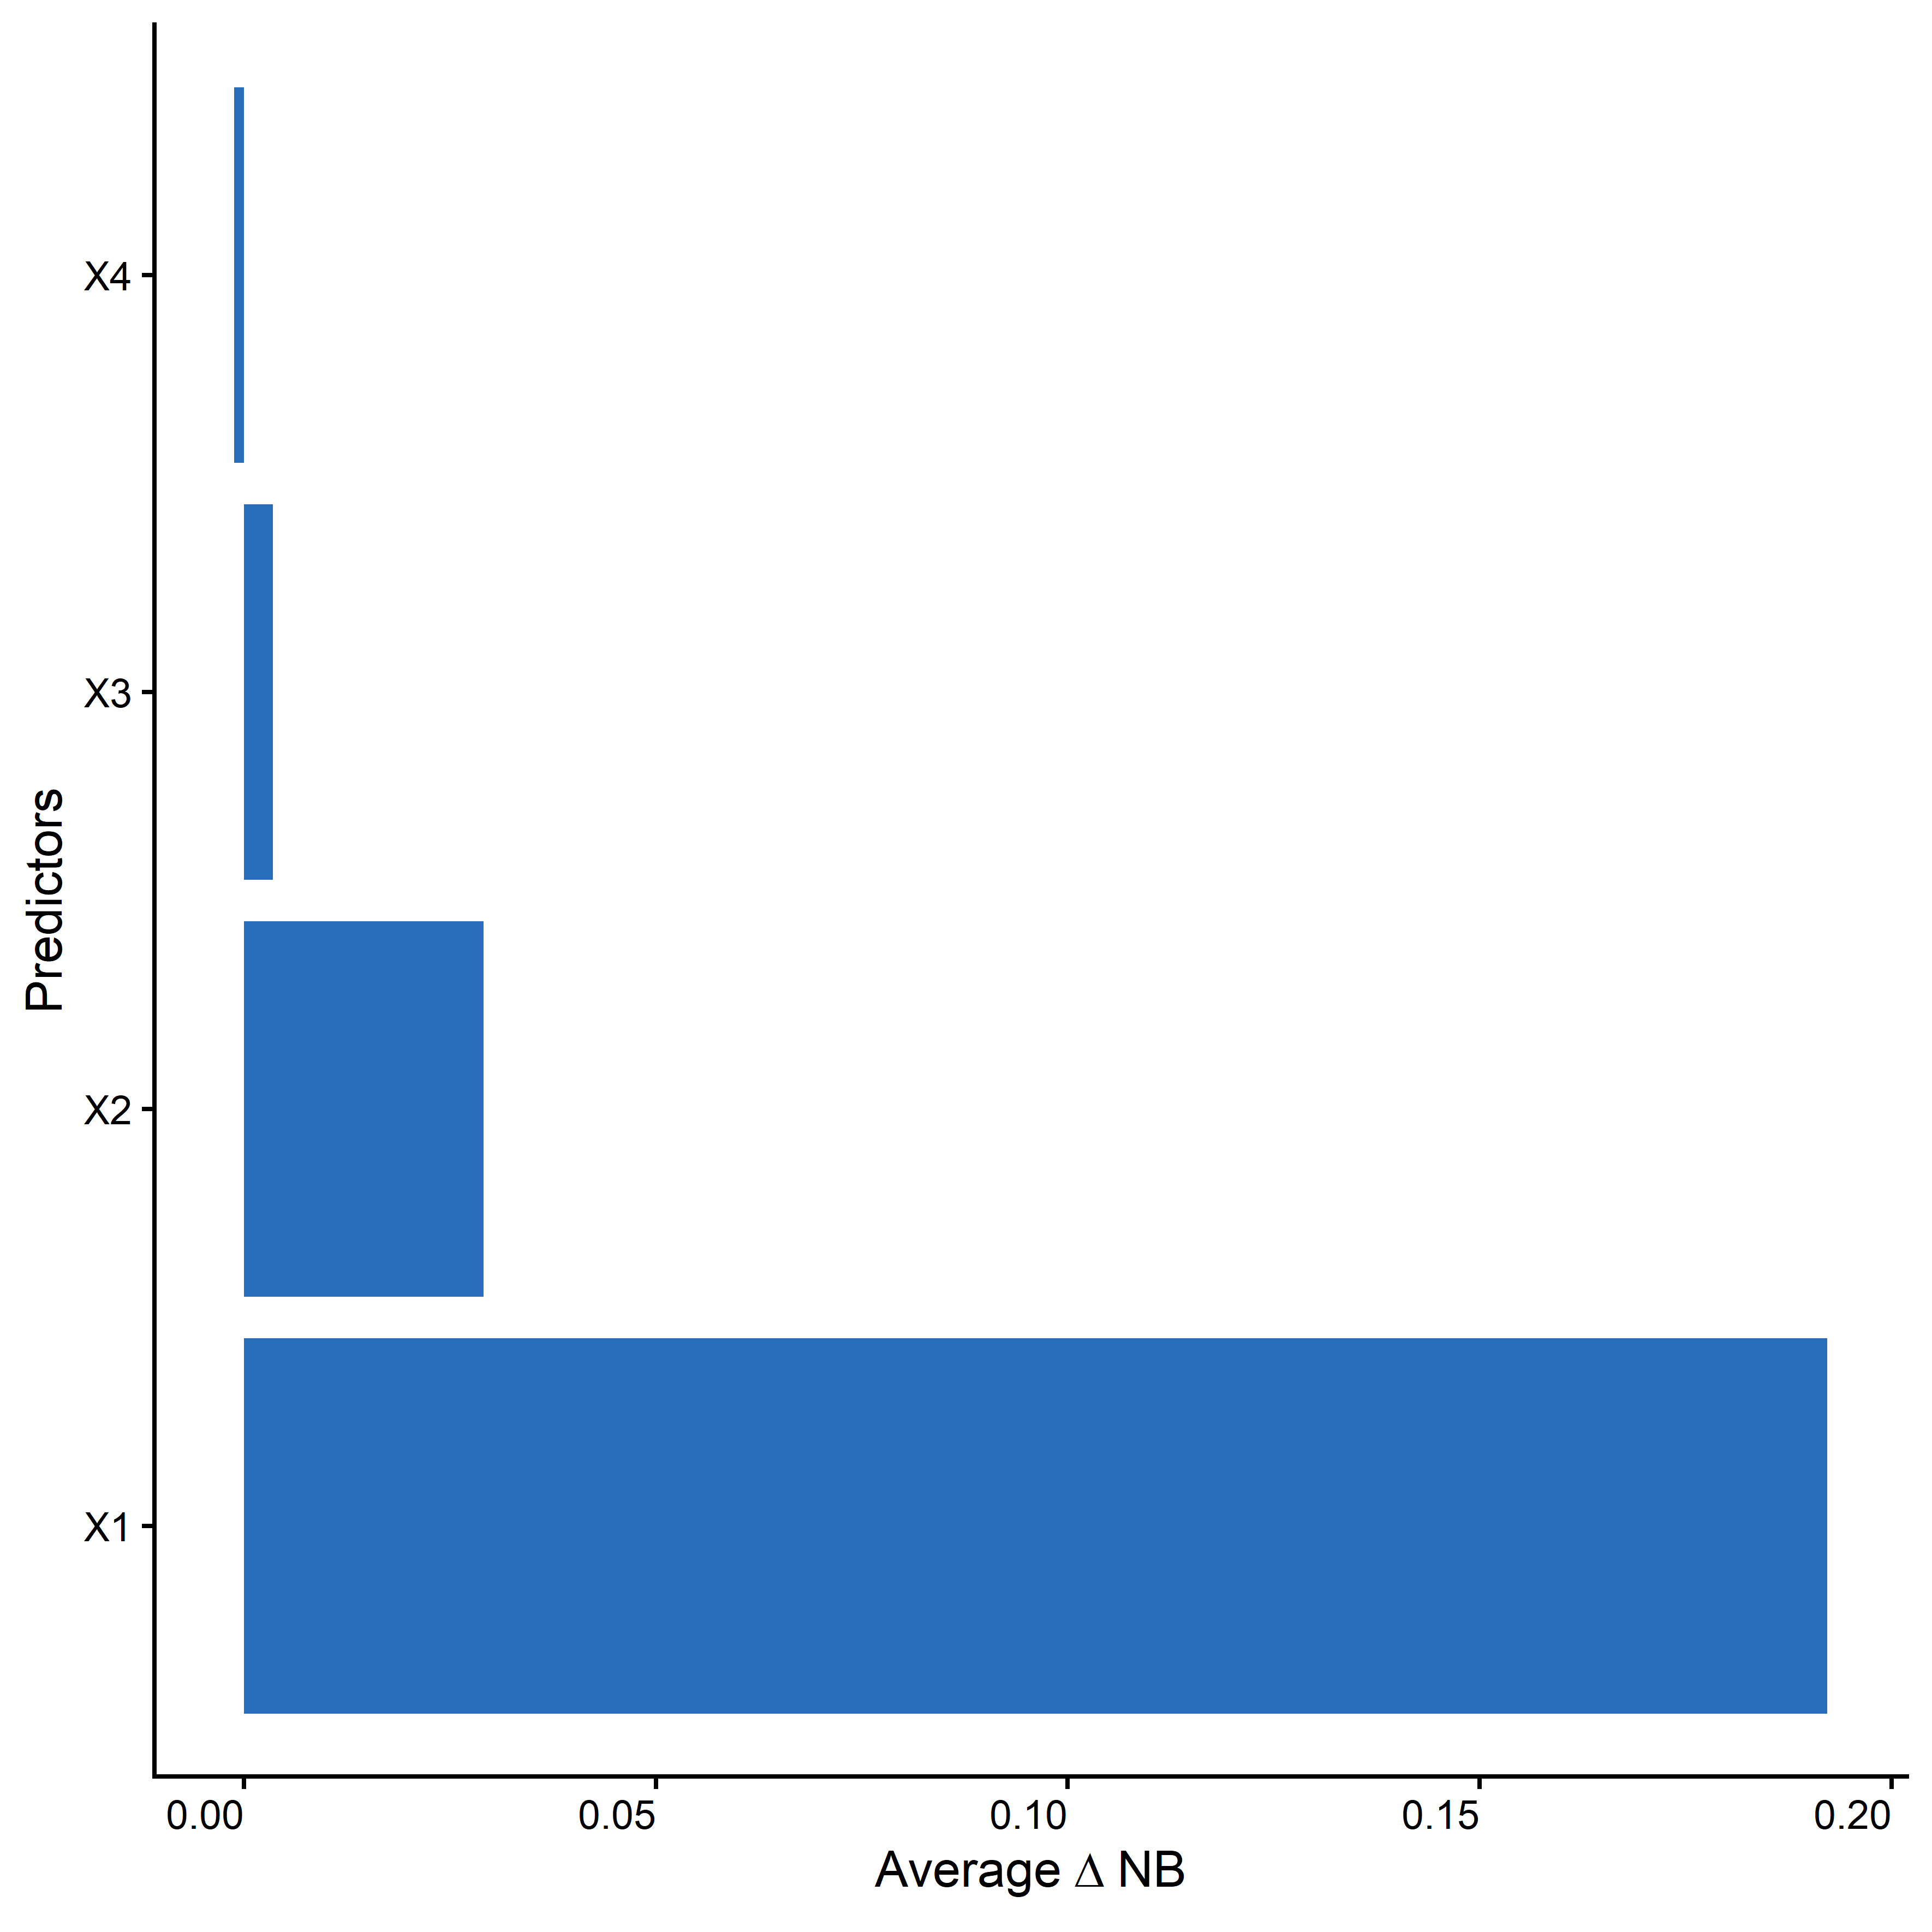
\includegraphics[width=\textwidth]{figures/varselection/fig-simple_illustration_train-1.png}
	\caption{Net benefit based variable importance for the simple illustration. NB: Net benefit.}
\end{subfigure}\hfill
\begin{subfigure}[t]{0.48\textwidth}
	\centering
	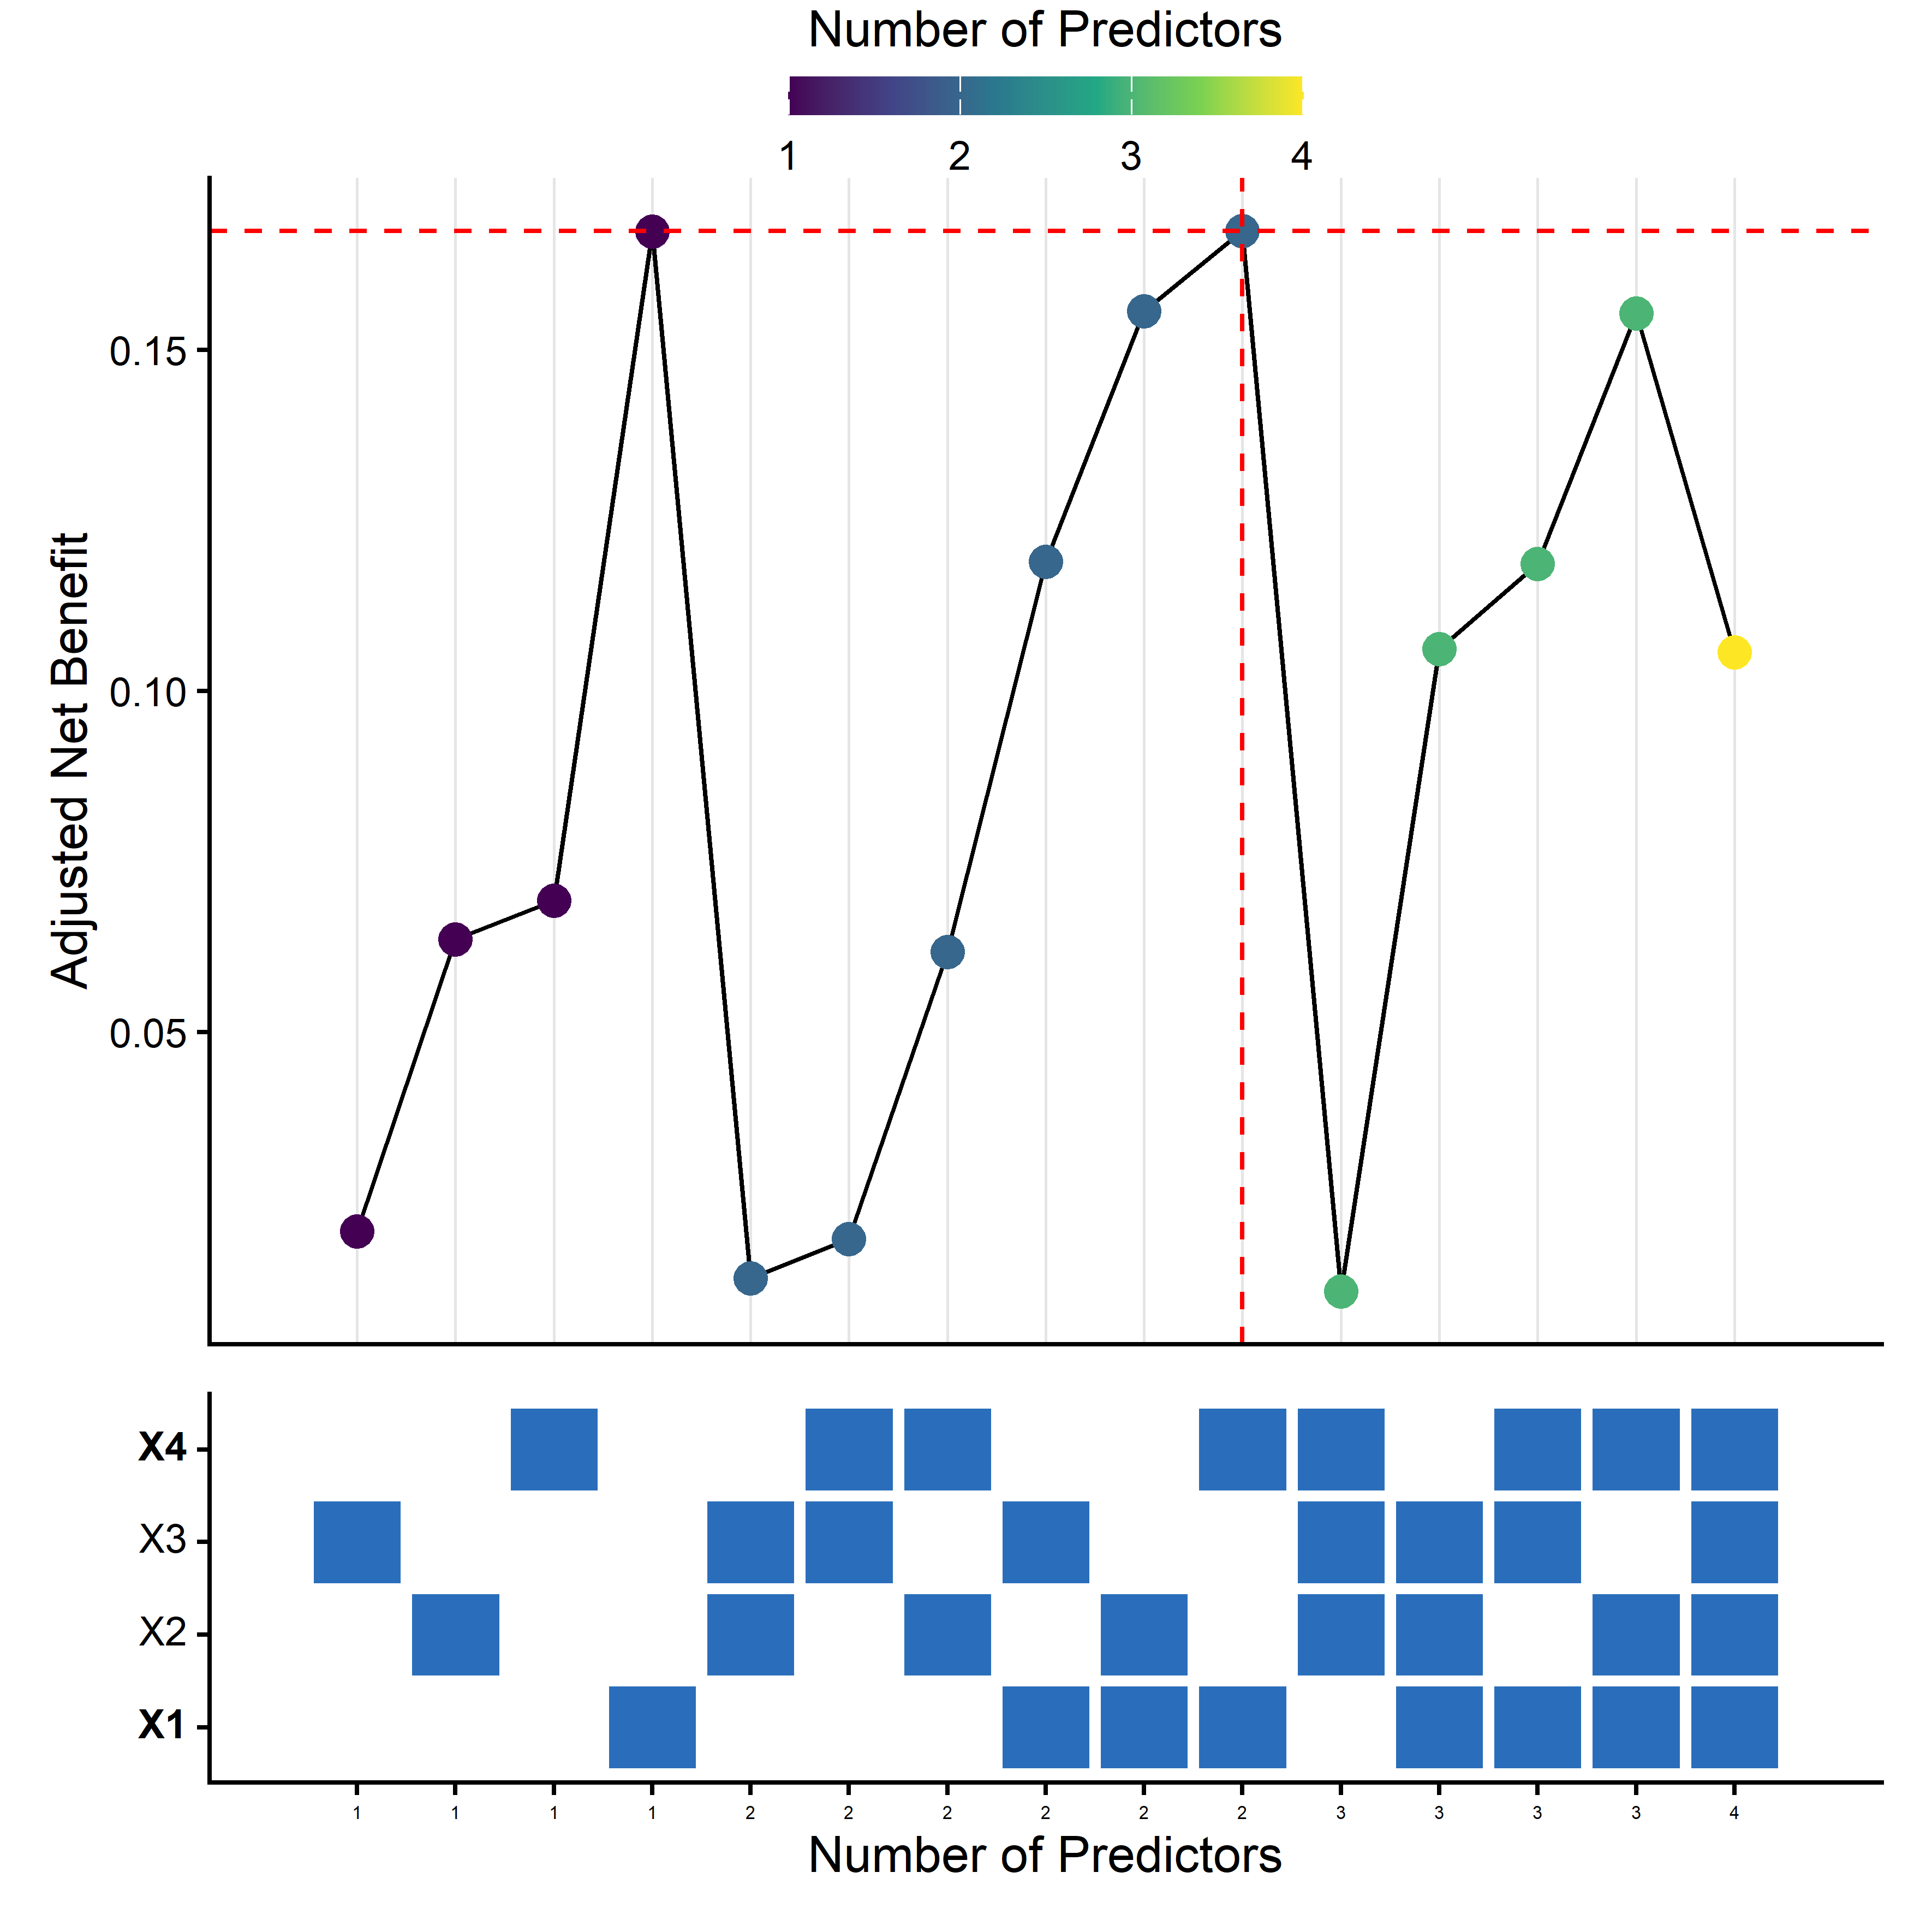
\includegraphics[width=\textwidth]{figures/varselection/fig-simple_illustration_train-2.png}
	\caption{All-subset plot for the simple illustration.}
\end{subfigure}
\label{fig:varsel:importance}
\end{figure}

This simple illustration serves as an example on how the best subset of predictors based on performance in statistical terms does not necessarily mean better cost-utility. Then, using the same data generating mechanism we generated a larger test dataset (N = 100,000) for the three possible models based on the variable selection procedure selected. Table~\ref{tab:varsel:models} presents the results of the three models in 1000 bootstrap samples. In Figure~\ref{fig:varsel:dca} we illustrate the harm adjusted decision curves (A) of the three models and flexible calibration curves (B) using restricted cubic splines as smoother. As expected, the best model according to the harm-adjusted NB is always the simpler model. The right plot illustrates that calibration for that model is slightly worse, showcasing the need to find a balance between statistical performance and decision-making.


% Placeholder for Figure 2 (Decision curve and calibration)
\begin{figure}[h!]
\centering
\begin{subfigure}[t]{0.48\textwidth}
	\centering
	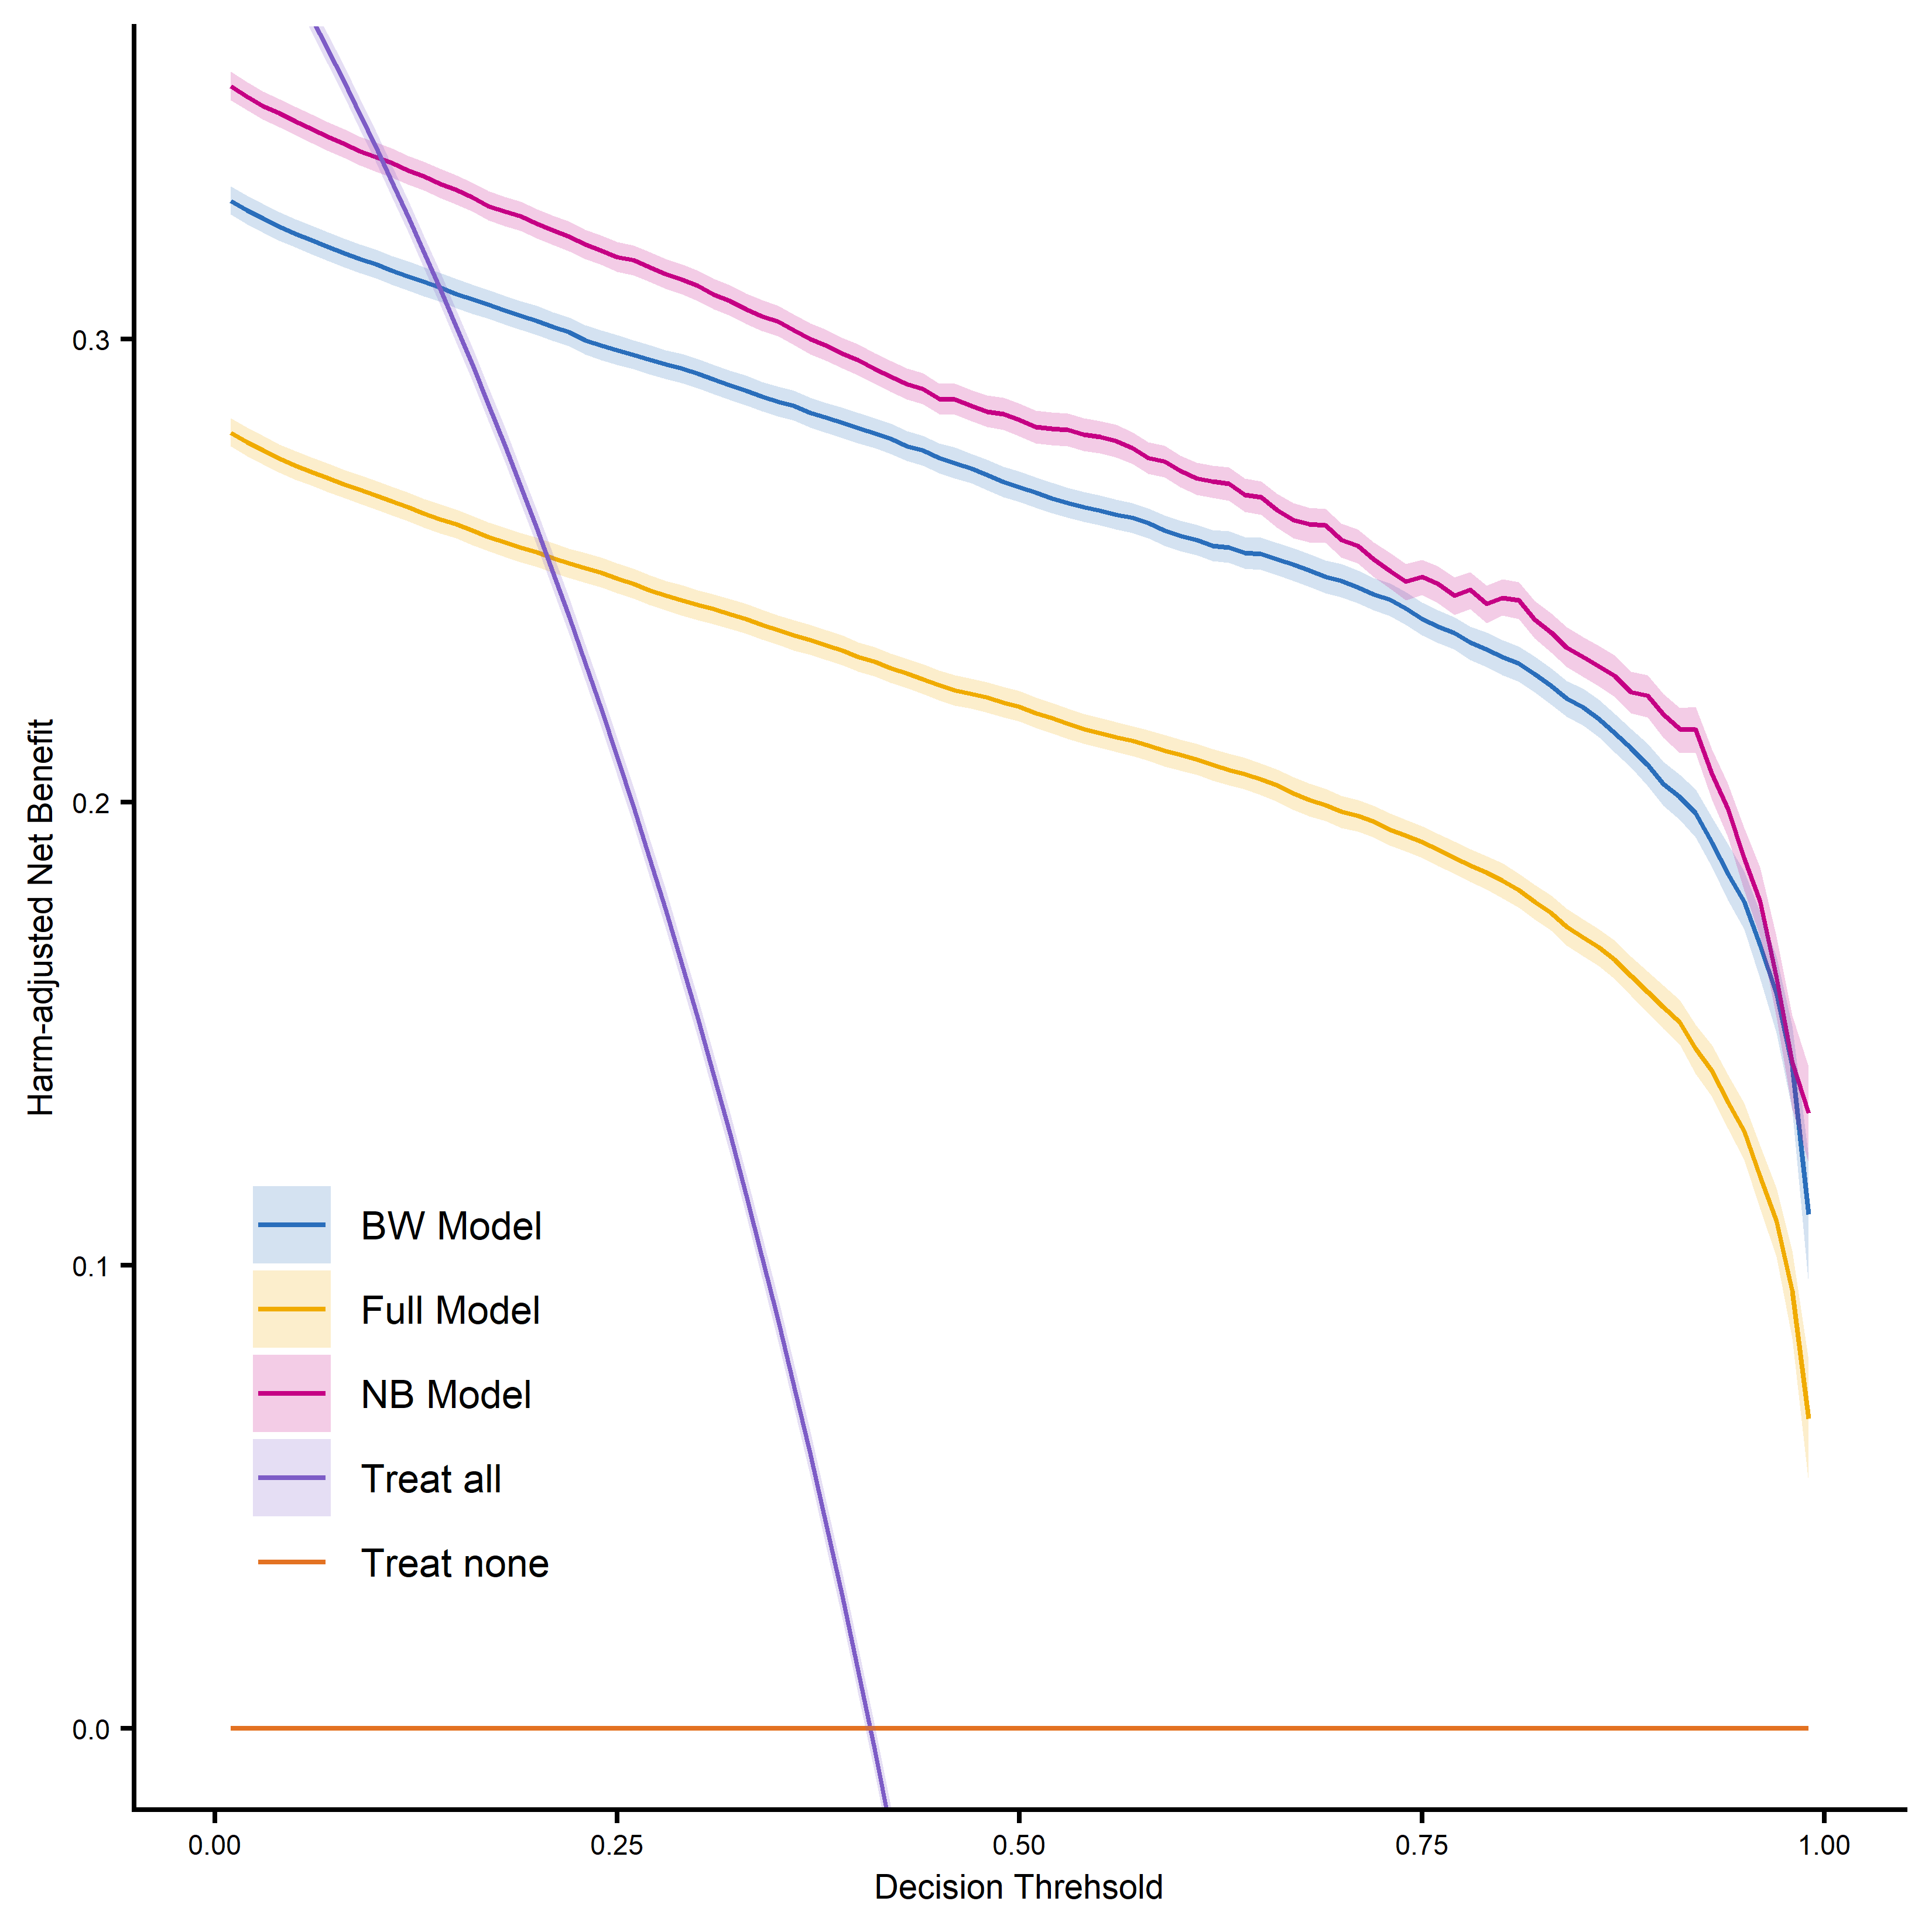
\includegraphics[width=\textwidth]{figures/varselection/fig-simple_illustration_test-1.png}
	\caption{Decision curve analysis for the simple illustration. NB: Net benefit.}
\end{subfigure}\hfill
\begin{subfigure}[t]{0.48\textwidth}
	\centering
	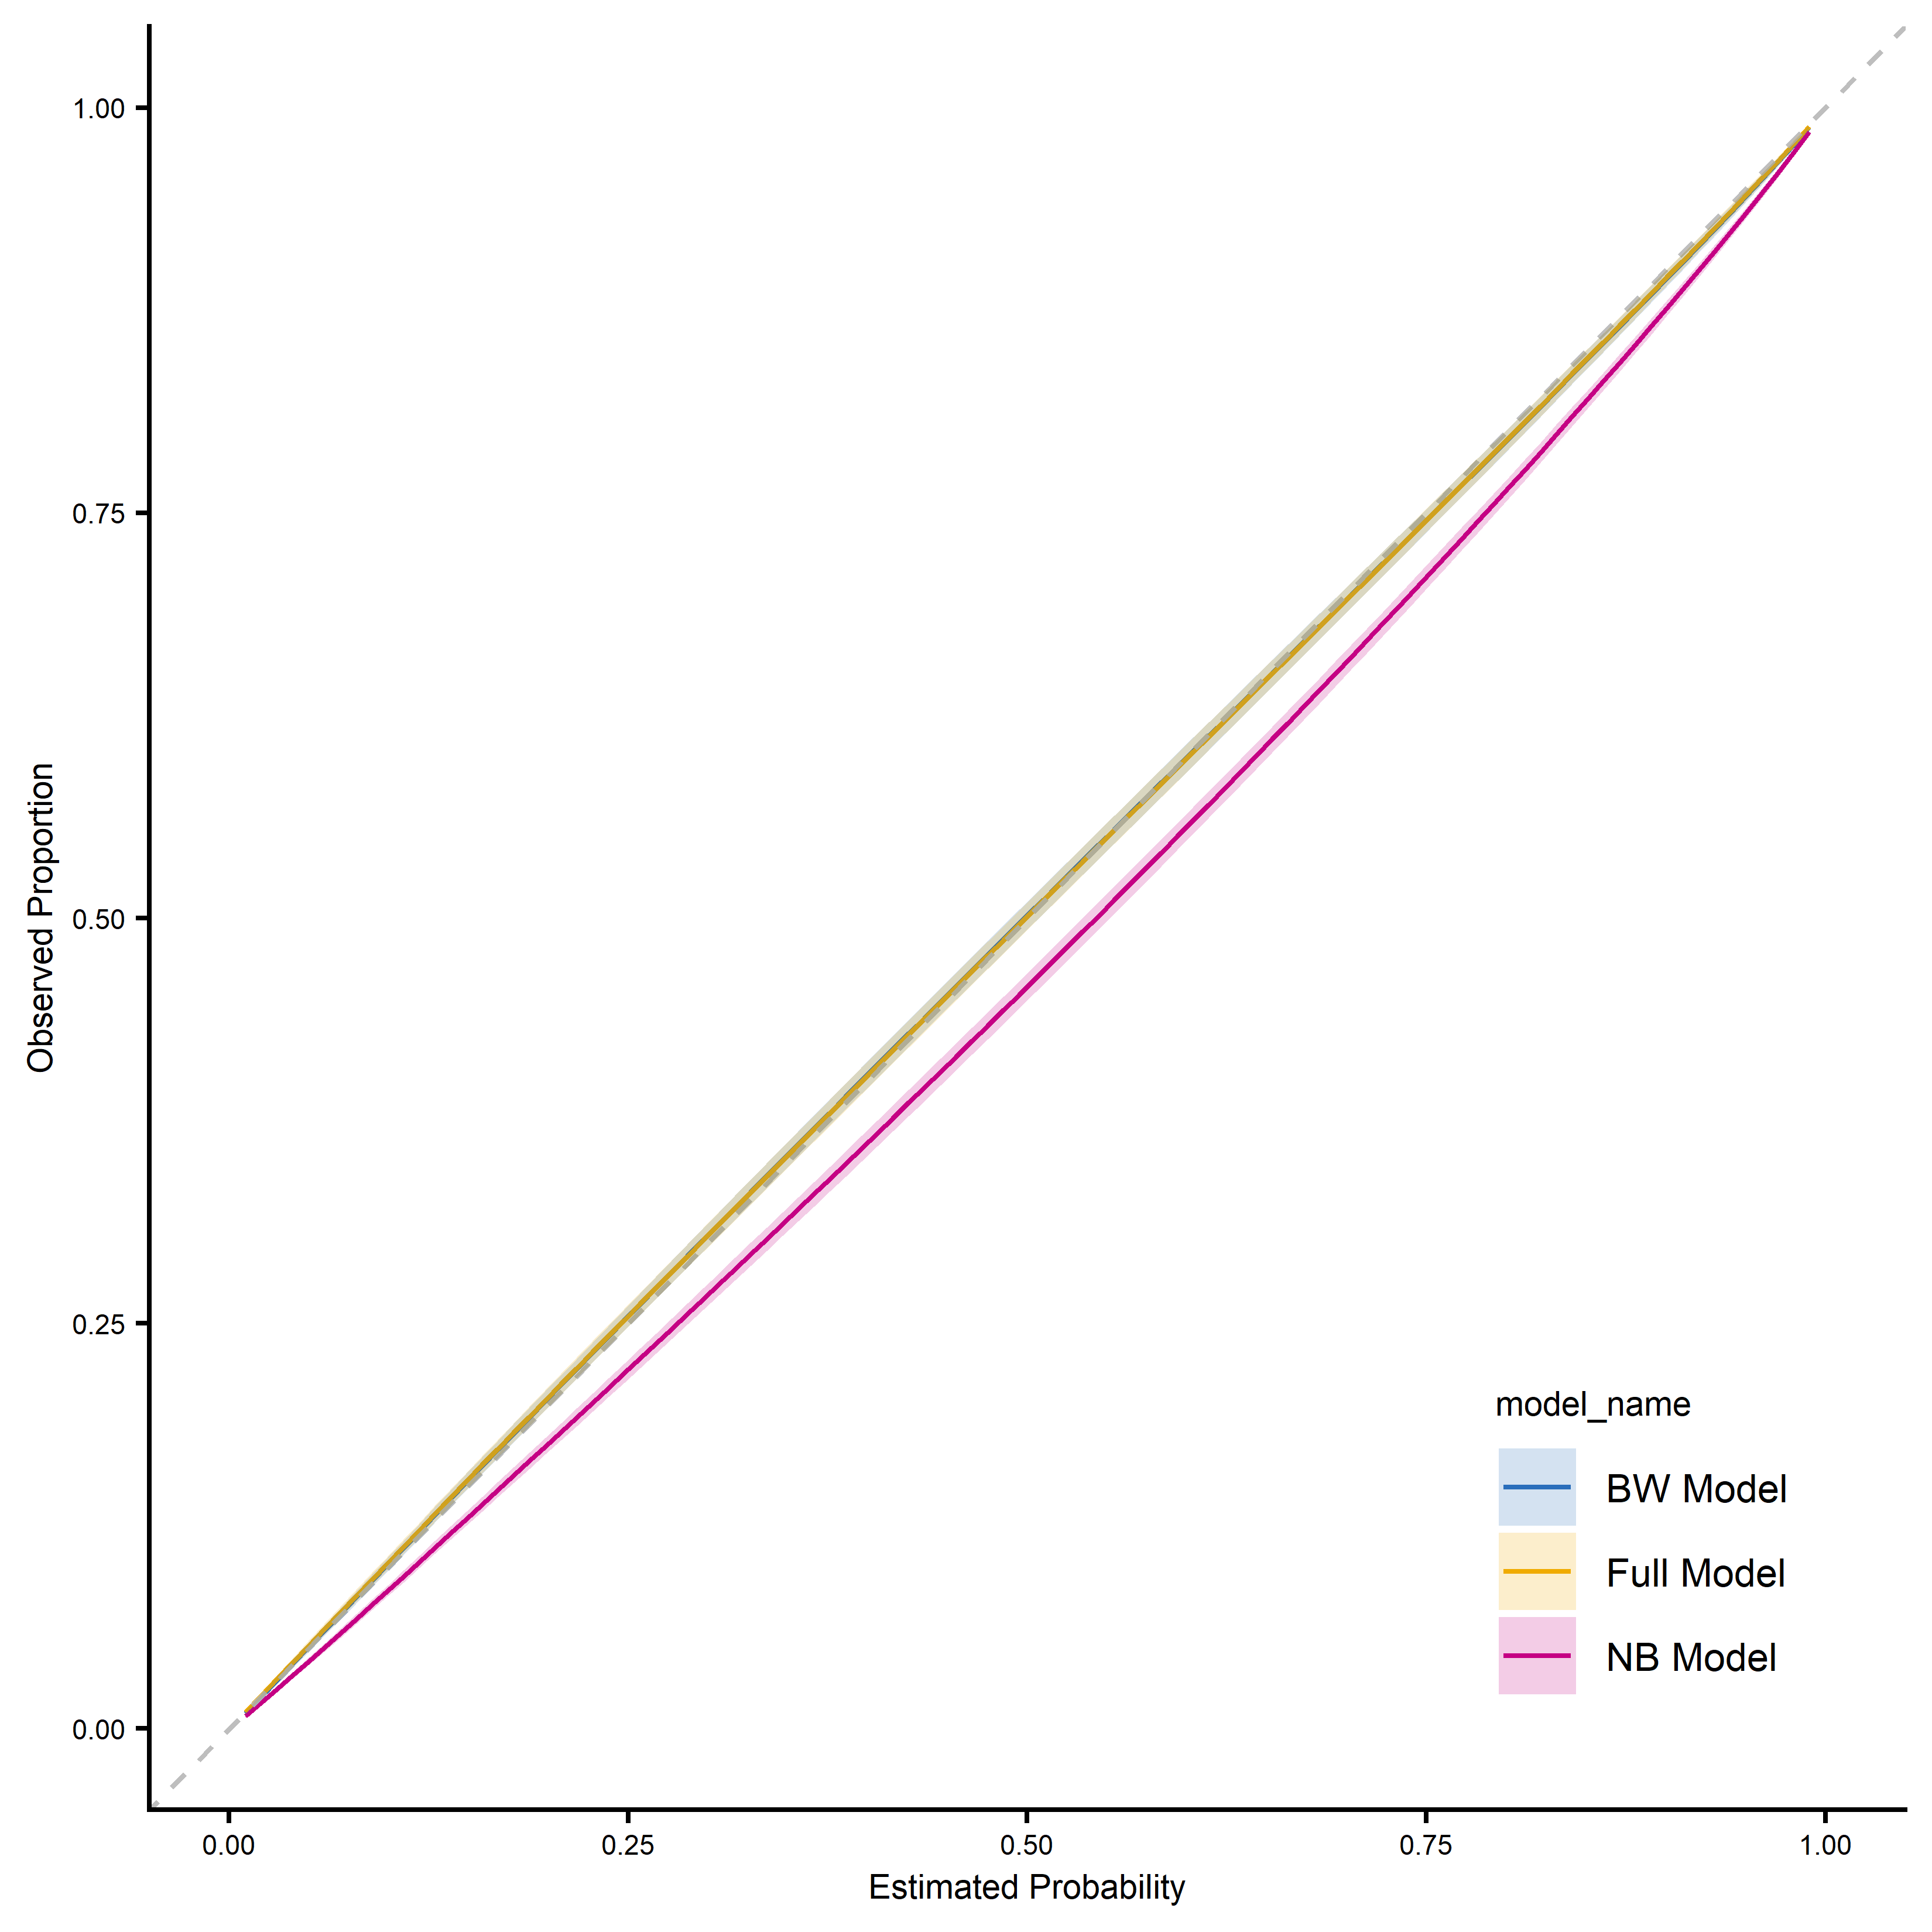
\includegraphics[width=\textwidth]{figures/varselection/fig-simple_illustration_test-2.png}
	\caption{Calibration plot for the simple illustration.}
\end{subfigure}
\label{fig:varsel:dca}
\end{figure}


\begin{table}[h!]
\centering
\small
\caption{Model comparison (mean ± 95\% CI over 1000 bootstraps on test set of 100k observations; NB threshold 10\%).}
\begin{tabularx}{\textwidth}{XXXXXXX}
\toprule
\textbf{Method} & \textbf{AUC} & \textbf{Brier} & \textbf{O:E} & \textbf{Net} & \textbf{Harm} \\
 & & & \textbf{ratio} & \textbf{Benefit} & \textbf{Adj. NB} \\
\midrule
Backward elim. & 0.970 & 0.068 & 0.987 & 0.522 & 0.371 \\
Perform. (CV) & 0.974 & 0.064 & 0.990 & 0.522 & 0.361 \\
Net Benefit & 0.966 & 0.074 & 0.974 & 0.522 & 0.421 \\
\bottomrule
\end{tabularx}
\label{tab:varsel:models}
\end{table}

\section{Case studies}

We will test the variable selection methodology with three datasets previously used to develop clinical prediction models. We will then compare the performance in terms of discrimination (AUC), calibration (calibration plots) and clinical utility (Net Benefit and DCA).

The analysis was performed on an HP EliteDesk 8 Tower G11 Desktop AI PC equipped with an Intel Core Ultra 9 285 processor (24 cores, base frequency 2.50 GHz) and 128 GB of RAM, running on a 64-bit Windows operating system and with R version 4.4. The parallelized processes used 23 cores.

\subsection{Ovarian cancer diagnosis -- IOTA data}

The optimal management of patients with an ovarian tumour depends on the histology of the mass. Benign masses do not always need to be removed and can be monitored with ultrasound follow up  \cite{carleyLaparoscopyLaparotomyManagement2002}. According to a recent study with 2 year follow-up, most of these masses spontaneously resolve, which reduces the risk of surgical complications  \cite{froymanRiskComplicationsPatients2019}. If the mass is malignant, management in specialised oncology centers is suggested \cite{timmermanESGOISUOGIOTA2021}. The IOTA group has developed and implemented several prediction models that use ultrasound and clinical characteristics to estimate the risk of malignancy of ovarian masses preoperatively  \cite{kaijserImprovingStrategiesDiagnosing2013}. In 2014, the ADNEX model was published using data from the IOTA phases 1-3 (N = 5909) Van Calster et al. (2014) \cite{vancalsterEvaluatingRiskOvarian2014}. The model has shown excellent performance across different settings and populations, as shown in recent systematic reviews and meta-analyses \cite{bbarrenadaADNEXRiskPrediction2024,barrenadaHeadHeadComparison2025}. ADNEX is a multinomial model that predicts the risk of benign, borderline, stage I invasive cancer, stage II-IV invasive cancer or metastatic cancer. In this work, we will treat it as a binary model, where the risk of malignancy is equal to the sum of the four malignant subtypes. As a validation dataset we will use IOTA phase 5 study (N = 6847) which was prospectively collected to externally validate ADNEX  \cite{vancalsterValidationModelsDiagnose2020}.

The variable selection procedure is detailed in the supplementary material of the original publication \cite{vancalsterEvaluatingRiskOvarian2014}, we refer the reader there for details. The original ADNEX model utilized nine predictors: three clinical (age, serum CA125, and center type) and six ultrasound-based (lesion diameter, solid tissue proportion, >10 cyst locules, number of papillary projections, acoustic shadows, and ascites). While family history was initially considered, it was excluded during the variable selection process. For our analysis, missing CA125 values were handled via a regression-based imputation using all other ADNEX predictors, following recent methodological recommendations \cite{siskImputationMissingIndicators2023}. Then this model was applied to the development and validation dataset to impute missing values. In the validation dataset, some of the tumours were classified as uncertain for various reasons. In the published validation study, these values were also imputed with multiple imputation. We use those imputed values for our analysis.

We extended the original predictor set with five additional features: bilateral masses, irregular internal cyst walls, Doppler color score, maximum solid component diameter, and lesion-associated pain. In total 65,536 predictor combinations were evaluated across decision thresholds from 1\% to 20\% risk with 20-fold cross validation. We then compute discrimination in terms of AUC, clustered calibration and decision curve analysis \cite{barrenadaClusteredFlexibleCalibration2026}. Adjusted NB was also calculated with costs based on three group of variables: clinical history variables (no cost, should be available for all patients from the records), ultrasound based variables (TT = 200), blood based variables (TT = 80). We compared NB based variables selections to LASSO and backward elimination. The total time to run the algorithm was 1h 25 minutes.

All models removed family history of ovarian cancer. The LASSO model also removed presence of papillary projections. NB based models removed instead maximum diameter of the solid part of the tumour and in addition the adjusted NB removed CA125 biomarker. According to the variable importance calculations, the least important predictor was family history and the most important one was the proportion of solid tissue.

The models showed comparable performance, with BE and NB-based approaches outperforming slightly the rest. Clinical utility of all models was similar, as shown in the decision curves, but when the costs of measuring a predictor are accounted for, the variable selection with adjusted NB was clearly more useful across the whole range of decision thresholds.

% Placeholder for Table showing IOTA results
\begin{table}[h!]
\centering
\small
\caption{IOTA variable selection comparison (VS = procedure, BE = backward elimination, Fam hist = family history, Pap = papillary projections, MSD = max solid diameter, Adj = adjusted).}
\begin{tabularx}{\textwidth}{XXXXXX}
\toprule
\textbf{VS Procedure} & \textbf{Removed} & \textbf{AUC} & \textbf{O:E} & \textbf{NB} & \textbf{Adj} \\
 &  & & \textbf{ratio} & \textbf{(10\%)} & \textbf{NB} \\
\midrule
BE & Fam hist & 0.961 & 0.957 & 0.226 & 0.209 \\
LASSO & Fam hist, Pap & 0.953 & 0.929 & 0.223 & 0.205 \\
NB & Fam hist, MSD & 0.961 & 0.974 & 0.227 & 0.209 \\
Adj NB & Fam hist, CA125 & 0.960 & 0.968 & 0.226 & 0.219 \\
\bottomrule
\end{tabularx}
\label{tab:varsel:iota}
\end{table}

% Placeholder for DCA figure
\begin{figure}[h!]
\centering
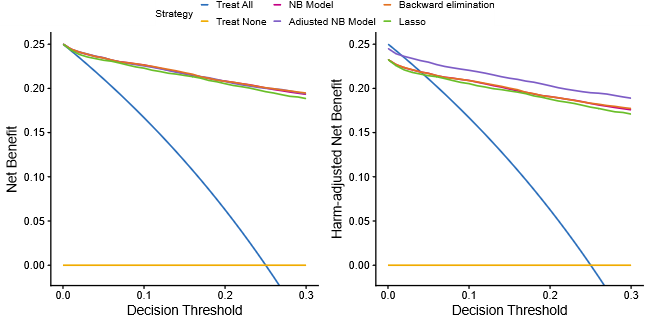
\includegraphics[width=0.8\textwidth]{figures/varselection/ADNEX_dca.png}
\caption{Decision curve analysis for unadjusted (left) and harm-adjusted (right) for the different variable selection procedures (IOTA ovarian cancer data).}
\label{fig:varsel:iota}
\end{figure}

\subsection{Emergency department hospitalization -- MIMIC IV ED (Large dimensional setting)}

For the second case study we will use the well-known MIMIC IV emergency department (MIMIC IV ED) data combined with the MIMIC IV to predict the risk of hospitalization after visiting the emergency department \cite{PhysioNet-mimiciv-3.1,hysioNet-mimic-iv-ed-2.2,johnsonMIMICIVFreelyAccessible2023}. MIMIC IV ED contains electronic health records data collected retrospectively from more than 425,000 emergency department stays in the Beth Israel Deaconess Medical Center in Boston, between 2011 and 2019. We use the benchmark proposed by Xie et al., but with the latest version of MIMIC IV (v3.1) and MIMIC ED (v2.2) Xie et al. (2022) \cite{xieBenchmarkingEmergencyDepartment2022}. The authors propose this benchmark to allow different model developers to make fair comparisons when using MIMIC IV data, therefore we followed the same procedure to obtain the training and test data according to their guidelines. The training data contains 334,420 (80\%) patients and the testing data 83605 (20\%).

They propose 64 predictors to develop models to predict risk of hospitalization when a patient arrives to the emergency department, and they develop models using different algorithms, but we will focus on the LR model, that we denote as baseline model. The predictor distribution across test and training datasets is identical and is displayed in Table S6. If we were to use the exhaustive approach as in the ovarian cancer case this would mean approximately $2^{64}$ (million trillion) combinations, which obviously is not feasible. Therefore we will use the groupwise approach with group sizes 1 and 2.

The method with a group size of one completely ignores interactions between predictors, similar to backward elimination. In the first step, the algorithm trains 65 models, followed by 64 in the next step, and so on. For MIMIC IV-ED dataset, 8 predictors were removed using this algorithm and the process took 1.45 hours. The method with group size of two iteratively removes predictors in pairs, so it accounts for interactions of two predictors. This method is computationally more intensive because the algorithm needs to train 2017 models in first step, followed by 1953 and so on. In the data, the algorithm removed 12 predictors in 6 steps.

The most important predictors according to NB variable selection were triage acuity and age of the patient. Baseline model and groupwise approaches obtained similar AUC (0.81), but the groupwise approaches tended to obtain less extreme probabilities but consistently ranked slightly higher for clinical utility across the decision curve.

% Placeholder for Table showing MIMIC-ED results
\begin{table}[h!]
\centering
\footnotesize
\caption{MIMIC-ED variable selection comparison (Pred. = predictors, Mean NB = mean net benefit).}

\begin{tabularx}{0.6\textwidth}{XXXXX}
\toprule
\textbf{Method} & \textbf{Pred.} & \textbf{AUC} & \textbf{Time} & \textbf{Mean NB} \\
 & \textbf{Removed} & & & (20--80\%) \\
\midrule
Baseline & 0 & 0.810 & -- & 0.234 \\
Groupwise (1) & 8 & 0.811 & 1.45h & 0.241 \\
Groupwise (2) & 12 & 0.809 & 1.17d & 0.239 \\
\bottomrule
\end{tabularx}
\label{tab:varsel:mimic}
\end{table}

% Placeholder for Calibration plot
\begin{figure}[h!]
\centering
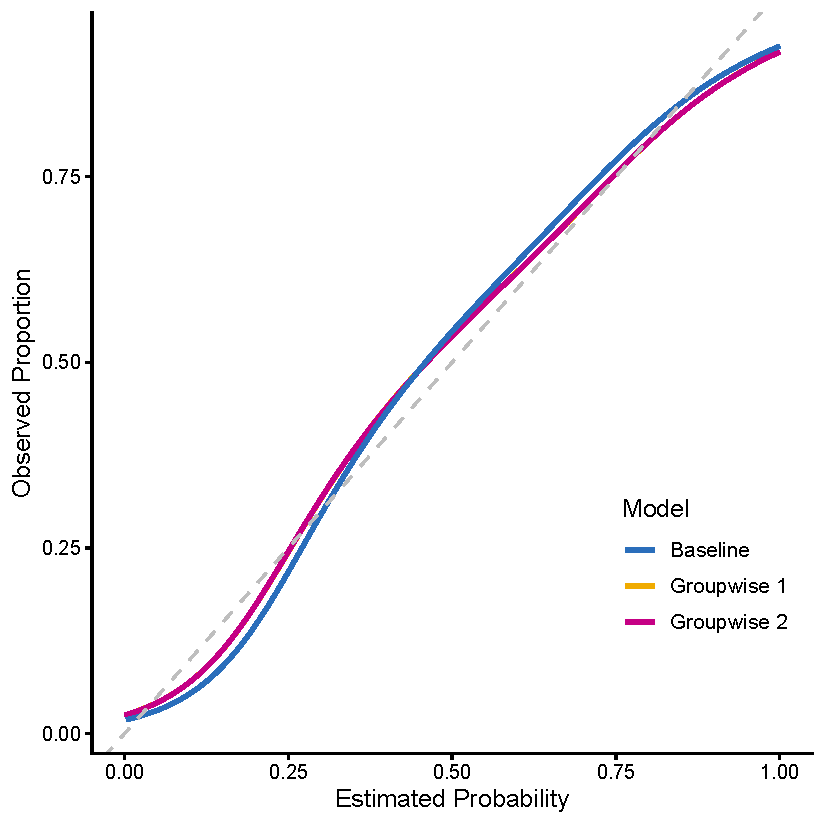
\includegraphics[width=0.8\textwidth]{figures/varselection/calibration_groupwise_mimic.pdf}
\caption{Calibration plot for the MIMIC-ED case study. Calibration for groupwise 1 and 2 are fully overlapping. (Results: Groupwise 1 time 1.458248 hours, Groupwise 2 time 1.165657 days)}
\label{fig:varsel:mimic}
\end{figure}

\subsection{Non typhoidal Salmonella (NTS) - DeNTS trial}

The last case study will use prospective cohort data to predict the risk of non-typhoidal Salmonella (NTS) bloodstream infection in children under five to guide the choice of empirical antibiotics  \cite{tackDevelopingClinicalPrediction2025}. The dataset contains clinical information collected prospectively from 2,327 paediatric hospital admissions with severe febrile illness at the Kisantu district hospital in the Democratic Republic of Congo. We use the a priori clinical predictors proposed by Tack et al., applying their exact variable definitions and restricted cubic spline transformations for continuous predictors. The authors propose this specific set of predictors based on a systematic literature review to ensure clinical relevance and avoid data-driven bias; therefore, we followed the same procedure to obtain our variables according to their guidelines. They propose 11 predictors to develop models for antibiotic triage, and they develop a simplified clinical scoring system alongside it, but we will focus on their main multivariable logistic regression (LR) model.

In their work, variables were selected using a double backward elimination process and the final model was fitted using Firth's correction  \cite{puhrFirthsLogisticRegression2017}. We will compare their approach to the introduced net benefit variable selection including splines for continuous predictors and then fitting the final model also using Firth's correction. In our algorithm, continuous predictors were introduced either with splines or were removed. The authors propose the reasonable range of thresholds to be between 20\% and 50\% so this were the range of thresholds used in the variable selection procedure.

If we were to use the exhaustive variable selection approach as in previous case studies, this would mean evaluating exactly 2,047 combinations. No test data was available, therefore, we present apparent results first and then to correct for optimism and compare the published approach and our algorithm we repeated the process across 1000 bootstrap samples.

\subsubsection{Apparent performance}

According to NB variable selection, the model removed the age, malnutrition and hemoglobin levels. Individual risks varied considerably among the published model and the model where variables were removed. The calibration of the model was closer to the diagonal for the NB model for estimated risk below 45\% but tended to estimate too low risks in higher estimated probabilities. The model had higher NB from decision thresholds of 25\% till 55\%.

% Placeholder for Figure showing risk distribution
\begin{figure}[h!]
\centering
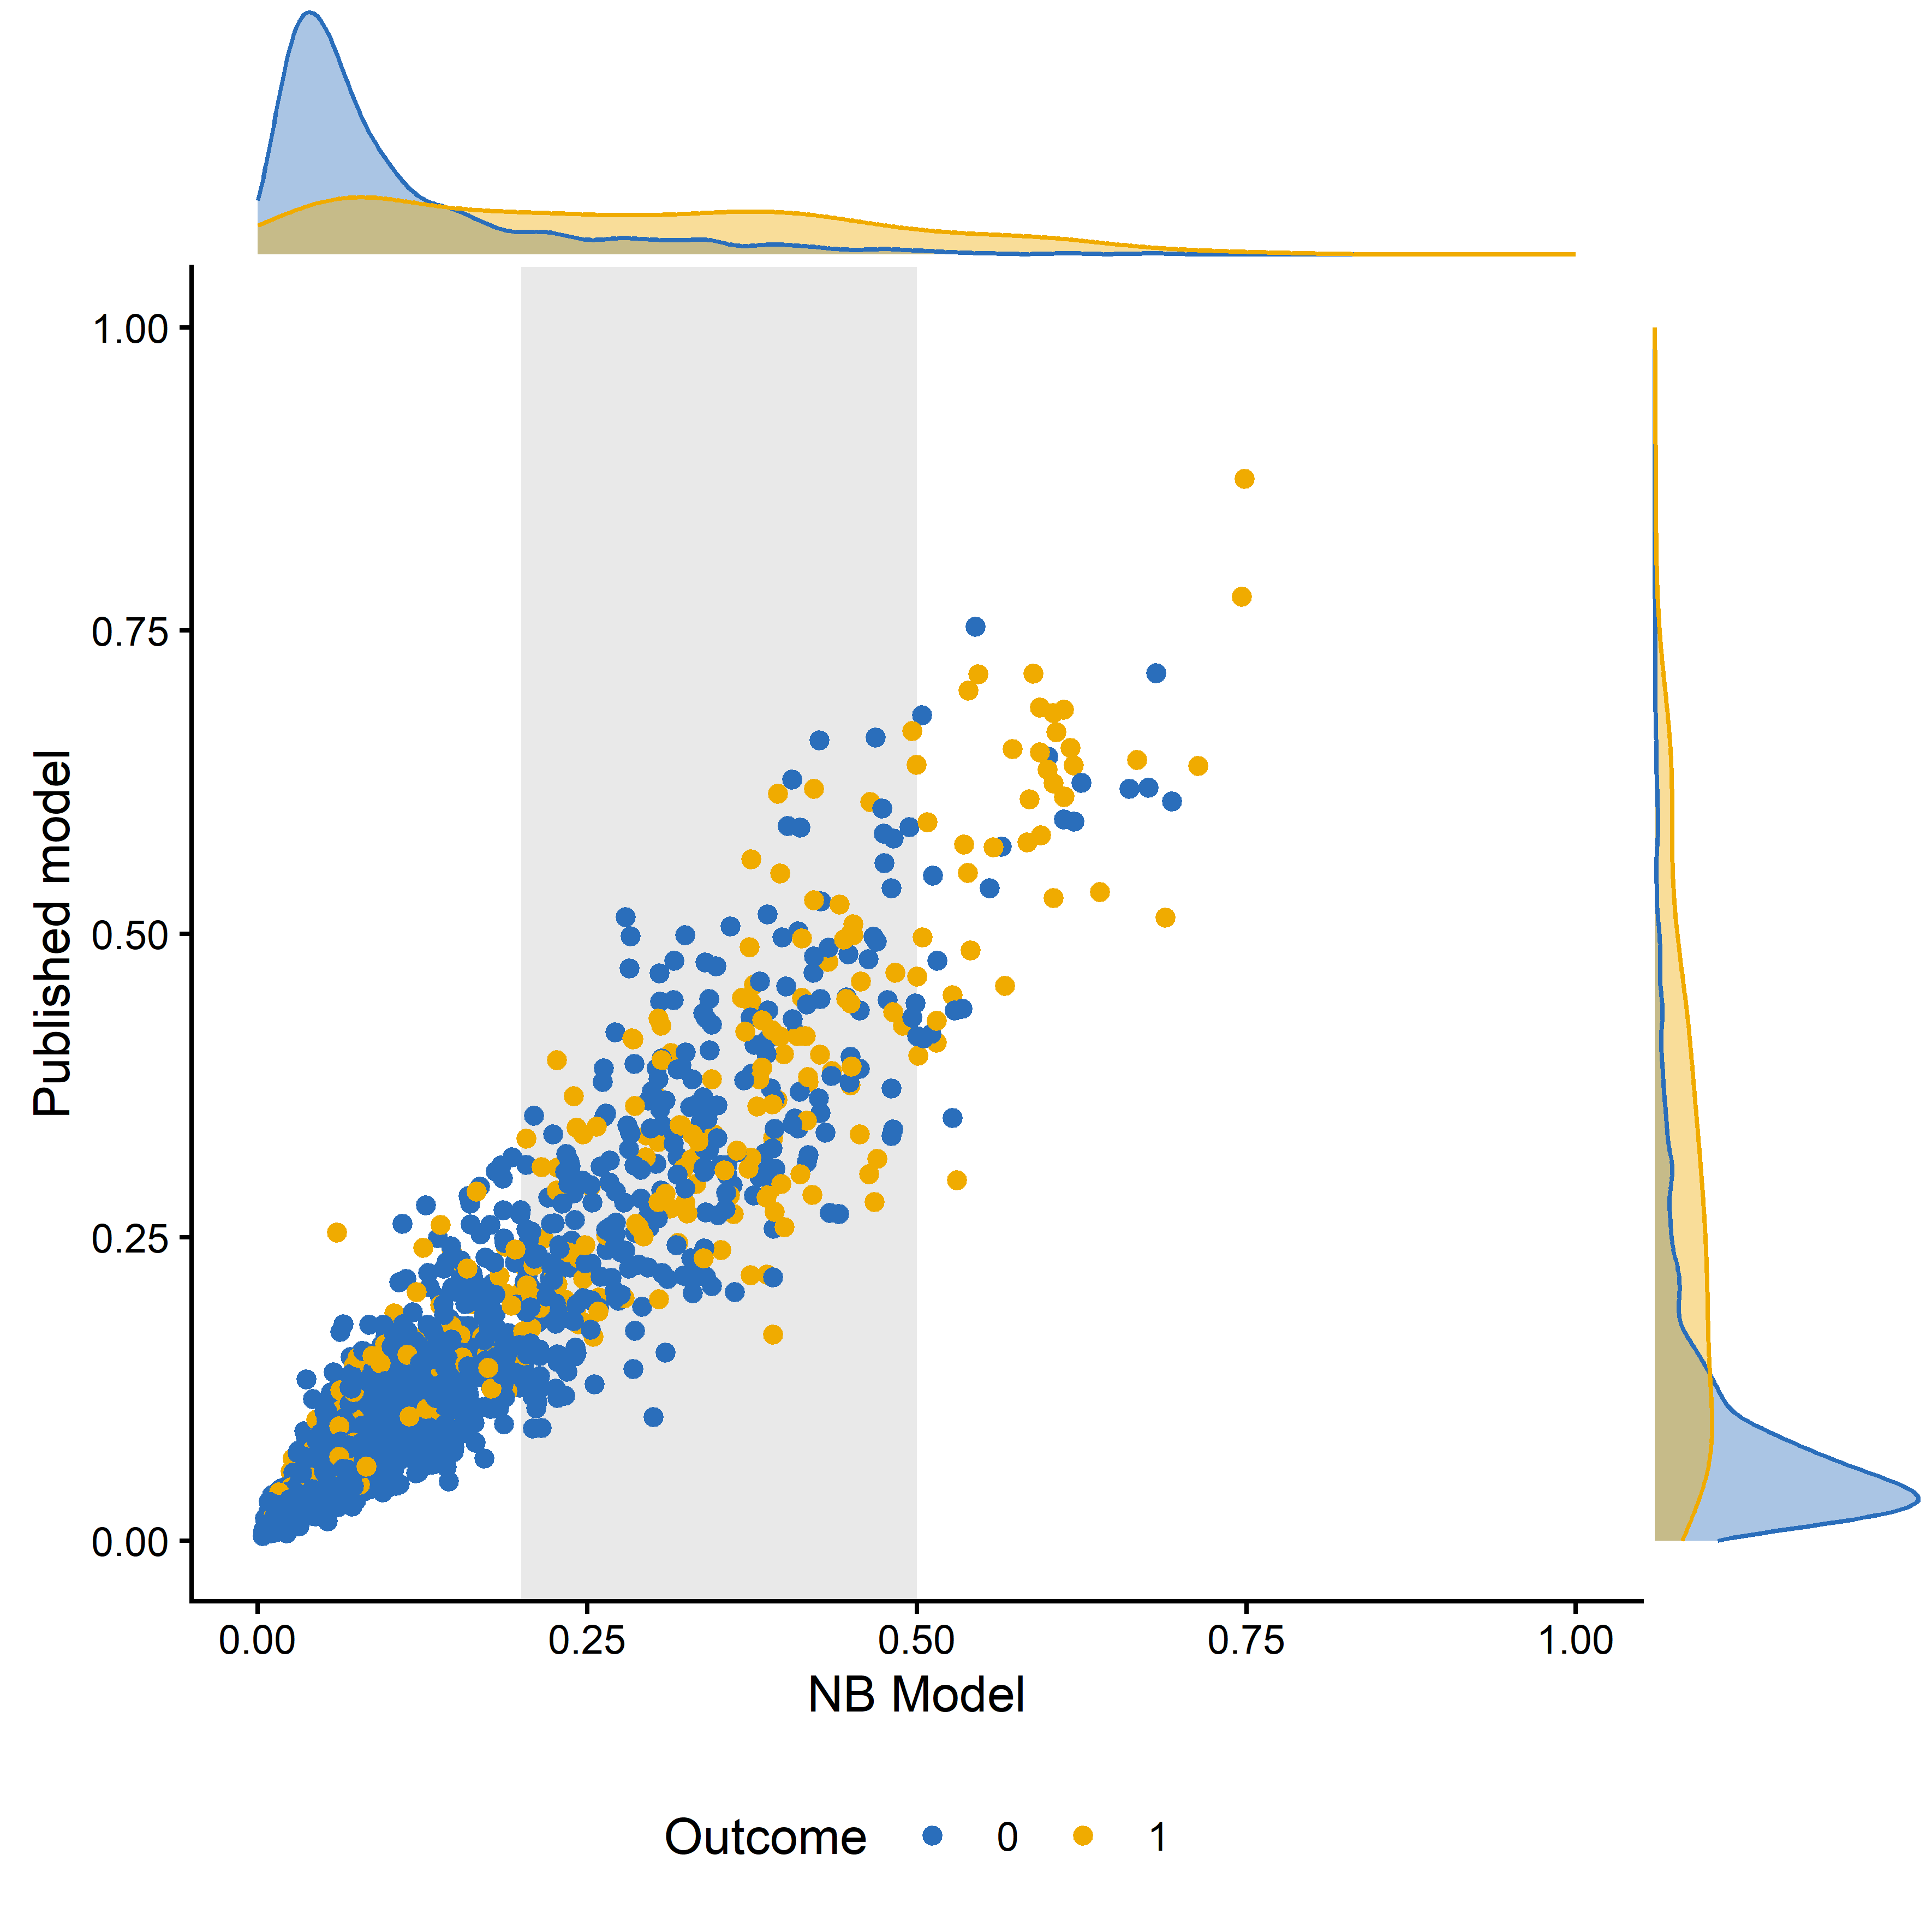
\includegraphics[width=0.8\textwidth]{figures/varselection/fig-auc_dents-1.png}
\caption{Distribution of individual risks for the model based on NB variable selection and the published model by outcome. Plots in the margin depict densities per outcome.}
\label{fig:varsel:dents}
\end{figure}

\subsubsection{Bootstrap results}

Discrimination and calibration metrics showed similar results for both models. However, the median net benefit across the reasonable range of decision thresholds was better for the NB based variable selection algorithm.

% Placeholder for Table showing DeNTS results
\begin{table}[h!]
\centering
\footnotesize
\begin{tabular}{lccc}
\toprule
\textbf{Metric} & \textbf{Published} & \textbf{NB} & \textbf{Diff} \\
 & \textbf{Model} & \textbf{Selection} & \\
\midrule
AUC & 0.784 & 0.791 & +0.007 \\
Calib. O:E & 0.991 & 0.995 & +0.004 \\
Mean NB & 0.156 & 0.167 & +0.011 \\
\bottomrule
\end{tabular}
\caption{DeNTS trial results (median Q1--Q3) across 1000 bootstrap runs; AUC = AUROC, Calib = calibration, NB = net benefit, Diff = difference.}
\label{tab:varsel:dents}
\end{table}

% Placeholder for optimism-corrected DCA figure
\begin{figure}[h!]
\centering
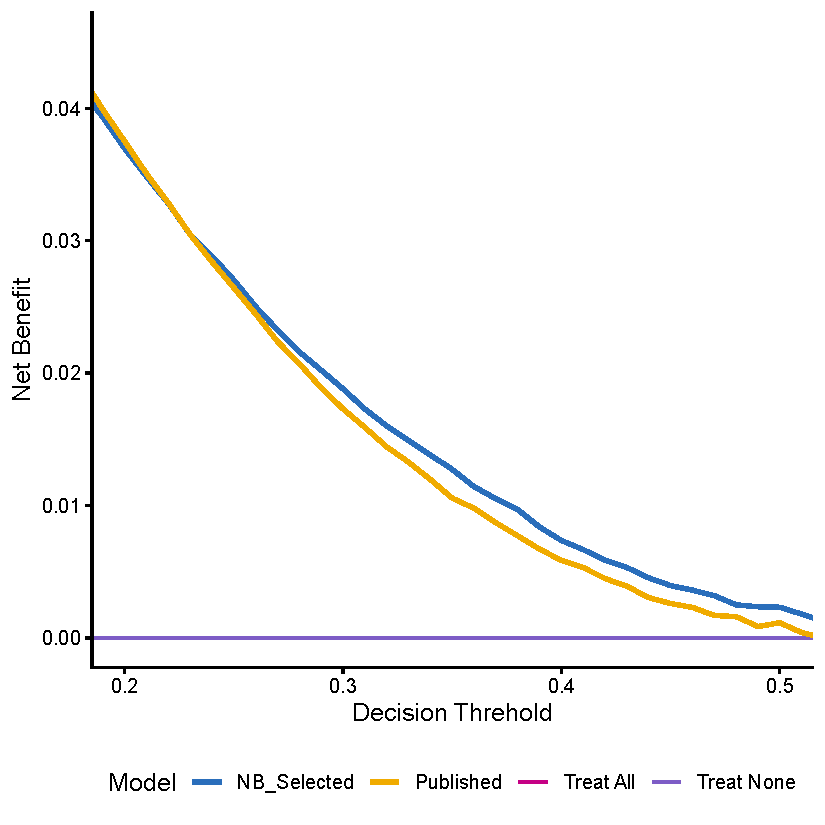
\includegraphics[width=0.8\textwidth]{figures/varselection/DCA_bootstrap_dents_zoomed.pdf}
\caption{Optimism corrected decision curve analysis based on 1000 bootstraps (Median results) for the DeNTS trial.}
\label{fig:varsel:dents_dca}
\end{figure}

\section{Discussion}

\subsection{Summary of Key Findings}

While classical statistical properties are widely used to build clinical prediction models, relying solely on them for variable selection often fails to optimise clinical benefit and to account for the real-world burden of measuring predictors. To address this gap, we developed and implemented a variable selection algorithm as an easy-to-use R package that determines the optimal subset of predictors by exhaustively exploring all predictor combinations and maximizing clinical utility, measured via (harm-adjusted) Net Benefit (NB). Through our simple illustration and three case studies, we showed that this decision analysis-based approach effectively reduces model complexity, maintaining comparable discrimination, calibration and clinical utility. In the ovarian cancer case study, adjusting for measurement harm successfully removed the CA125 biomarker, a test requiring a blood draw, while maintaining comparable performance to traditional backward elimination and LASSO methods. Furthermore, we showed that by using a groupwise elimination approach, this methodology can be successfully scaled to high-dimensional datasets like MIMIC IV-ED, yielding slightly higher clinical utility across decision thresholds compared to baseline models.

\subsection{Interpretation of Results}

The results highlight that the ``best'' model in purely statistical terms (e.g., maximizing AUC or AIC/BIC) is not necessarily the most useful model in clinical practice. Purely statistical metrics do not have the ability to balance correctly identified cases and harms of misclassifying a patient as done through NB. In addition our approach accounts for harms of measuring predictors as an crucial layer for variable selection. For instance, in our simulated illustration, ignoring test harms led to the inclusion of predictors that offered negligible improvements in NB at a disproportionate measurement cost. By translating the clinical burden into a Test Tradeoff, the minimum number of tests a doctor is willing to perform per true positive to justify the cost, our algorithm penalizes ``expensive'' predictors. Consequently, models developed using this algorithm are naturally more parsimonious and tailored for pragmatic clinical implementation, as seen in the DeNTS trial data where the NB-based model achieved a better median net benefit in the 25\% to 55\% threshold range while requiring fewer predictors.

\subsection{Contextualization Within Existing Literature}

There is growing recognition in the field of clinical prediction modelling that traditional performance measures are insufficient to guarantee a model's clinical value \cite{steyerberg2019clinical,calsterPerformanceEvaluationPredictive2024}. However, embedding utility directly into the variable selection phase has historically been difficult. While Baker et al. (2012) \cite{bakerEvaluatingNewMarker2012} discussed the use of Net Benefit to evaluate new markers, it was not operationalized as an automated variable selection algorithm. Previous attempts to introduce cost-based selection, such as the cost-adjusted Bayesian Information Criterion (BIC) proposed by Fouskakis and colleagues \cite{fouskakisBayesianVariableSelection2009}, struggled with complexity, requiring clinicians to specify difficult cost-penalized priors. Our approach bridges this methodological gap by anchoring the penalty to Net Benefit and the Test Tradeoff, providing a much more intuitive scale for clinicians to quantify the harm-to-benefit ratio.

\subsection{Limitations}

Despite its advantages, this methodology has several limitations:

\begin{enumerate}
\item Determining the specific ``harm'' of measuring a predictor is subjective, highly context-dependent, and challenging to quantify precisely prior to model development.

\item Because the method is a data-driven variable selection process, it is susceptible to overfitting, especially in studies with limited sample sizes. The procedure must strictly adhere to modern minimum sample size recommendations to prevent overly optimistic performance.

\item The exhaustive evaluation of all predictor combinations is computationally intensive and becomes infeasible with a large number of candidate predictors, though the proposed groupwise extension mitigates this issue.

\item For the moment, we only include logistic regression, but we aim to increase to other modelling algorithms.
\end{enumerate}

\subsection{Implications}

Prediction models that require burdensome, invasive, or expensive data collection for only marginal statistical gains are rarely adopted in routine care \cite{wyattCommentaryPrognosticModels1995}. By integrating clinical utility directly into the model training pipeline, developers can ensure that their final models are both statistically rigorous and practically viable. The open-source NBvarsel R package (\url{https://lasaibarrenada.github.io/NB_varsel/}) and its associated visualizations provide researchers with accessible tools to make informed, utility-driven decisions about variable selection.

\subsection{Future Research}

Future research should focus on extensive evaluation of the methodology under controlled setting with simulation studies and to extend the methodology to other modelling algorithms. For logistic regression, the methodology would also benefit of further utilities such as full control over variable interactions and spline terms. The package is intended to be continuously updated, and we made it open-source welcoming contributions from the community.

Another approach to account for clinical utility directly into parameter estimation could be using harm-adjusted NB as the optimization criterion for a loss function in deep learning architectures \cite{vickersHypothesisNetBenefit2025}.

\subsection{Conclusion}

Clinical utility should not be an afterthought reserved only for external validation. By integrating a harm-adjusted Net Benefit metric directly into the variable selection process, researchers can produce prediction models that maximize patient benefit while minimizing unnecessary clinical burden.

\glsunset{NB}
\glsunset{AUC}
\glsunset{BIC}
\glsunset{DCA}
\glsunset{TT}
\glsunset{EPV}
\glsunset{EPP}
